% The "%" character denotes a comment
% This file was written by Nathan Moore, Winona State University
% as a template for how lab reports might be written in LaTeX.
% style choices originally come from the American Journal of Physics's
% sample submission file, http://ajp.dickinson.edu/Contributors/manFormat.html
%
%
\documentclass[prb,preprint]{revtex4-1}
\usepackage{amsmath}  % needed for \tfrac, \bmatrix, etc.
\usepackage{amsfonts} % needed for bold Greek, Fraktur, and blackboard bold
\usepackage{graphicx} % needed for figures

%these are some macros (shortcuts)
\newcommand{\bea}{\begin{eqnarray}}
\newcommand{\eea}{\end{eqnarray}}
\newcommand{\be}{\begin{equation}}
\newcommand{\ee}{\end{equation}}

\begin{document}

\title{Electronics Lab 03: Operational Amplifiers}
\author{Adam Stammer}
%\email{adam.stammer@go.winona.edu}

\date{\today}

%if you include an abstract, it goes here
%\begin{abstract}
%Not Requested
%\end{abstract}

\maketitle


%These are my general reccomendations for an undergraduate lab report in Physics. 
%
%\textbf{Purpose}
%The lab report should start with a purpose statement.  Briefly 
%provide the necessary background and explain what problem your are trying to 
%solve/investigate.
%
%\textbf{Conclusions} Don't be coy, cut to the point right away and state what you found. This should be breif.
%
%\textbf{Theory} We never just measure stuff in Physics.  There's always a 
%theoretical idea behind the measurement we're making.  Explain  the ideas 
%behind your work, starting at the level of a successful Physics 221/222 
%student.
%
%\textbf{Data} Sketch out, in words and pictures, the apparatus you used to take data.  Report the data, graphically, if possible, and state the uncertainties  in your measurement.  Don't provide pages of computer printout here. Data tables shouldn't be your first choice when it comes to communicating your measurements.\cite{Tufte}
%
%\textbf{Analysis} With data presented, describe how the theory agrees/disagrees with 
%the data you took.  Normally this is accomplished with a fit line (or math 
%model) that is interpreted.
%
%\textbf{Limitations and Recommendations} Every measurement has limitations and it is only honest to report them to the reader.  ``Human Error'' is a meaningless statement.  After your analysis is complete, revisit the purpose statement.  This is the place to more forcefully argue your conclusions.    
%
%Notes: 
%Writing in the first person, eg ``I" or ``We," is fine.
%
%\newpage
%\textbf{Example Lab Report:}

\section{Purpose}
Not Requested  

\section{Conclusions}
Not Requested

\section{Theory}
There are multiple practical ways to hook up operational amplifiers. One of the most common is an inverting voltage amplifier. We can see a diagram of this below \ref{fig1}.

\begin{figure}[ht]
	\centering
	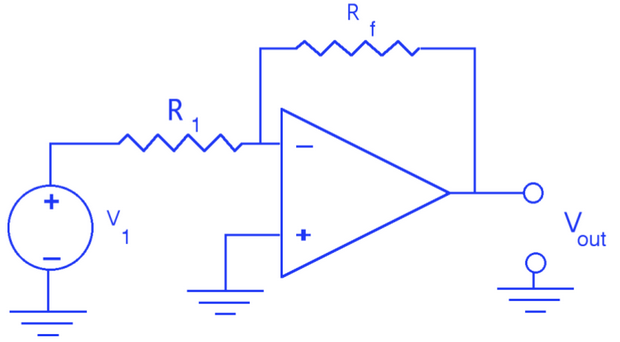
\includegraphics[width=3in]{circuit1.png}
	\caption{Inverting Voltage Amplifier}
	\label{fig1}
\end{figure}

Using nodal analysis we can find the output voltage $(V_{0})$. One of our golden rules of operational amplifiers states that no current flows in or out of the input terminals of the amplifier. Knowing this we can say that \ref{eq1}

\begin{equation}
I_{1} = I_{2}
\label{eq1}
\end{equation}

From here we can use Ohms Law [$I=\frac{V}{R}$] to say that

\begin{equation}
I_{f} = \frac{V_{o}-V_{-}}{R_{f}}
\label{eq2}
\end{equation}
\begin{equation}
I_{1} = \frac{V_{-}-V_{s}}{R_{1}}
\label{eq3}
\end{equation}

It's a simple matter of substitution from here. First we use our other golden rule to know that $V_{-}$ is equal to $V_{+}$ which is connected to ground. So the equation can be rewritten as seen below [\ref{eq4}].

\begin{equation}
\frac{V_{o}}{R_{f}} = \frac{-V_{1}}{R_{1}}
\label{eq4}
\end{equation}

Some simple algebra later and we'll have a practical equation to find $V_{o}$.

\begin{equation}
V_{o}=-V_{s}\frac{R_{f}}{R_{1}}
\label{eq5}
\end{equation}

We only need our golden rules to solve for $V_{o}$ in Circuit 2 [\ref{fig2}].

\begin{figure}[ht]
	\centering
	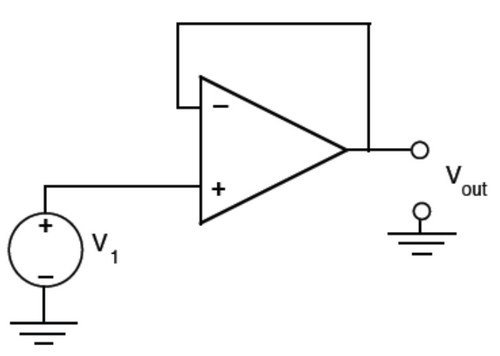
\includegraphics[width=3in]{circuit2.png}
	\caption{Voltage Follower Circuit}
	\label{fig2}
\end{figure}

\begin{equation}
V_{o}=V_{1}
\label{eq6}
\end{equation}


With a very similar process as with Circuit 1 [\ref{fig1}] we can solve Circuit 3 [\ref{fig3}].

\begin{figure}[ht]
	\centering
	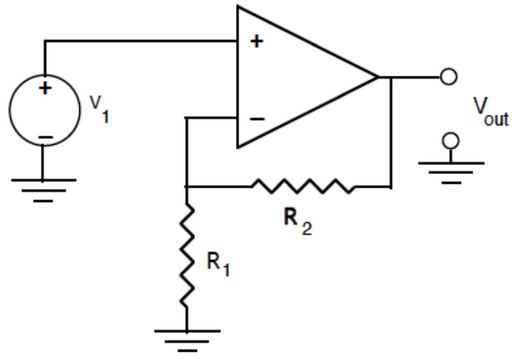
\includegraphics[width=3in]{circuit3.png}
	\caption{Non-Inverting Voltage Amplifier}
	\label{fig3}
\end{figure}

\begin{equation}
V_{o}=V_{1}\frac{R_{2}+R_{1}}{R_{2}}
\end{equation}

\section{Data}
Not Requested

\section{Analysis}
Taking the data gathered from one of our circuits we can graph it and look for a useful pattern or trend. The data taken from the voltage follower can be seen graphed in a scatter plot below [\ref{fig4}].

\begin{figure}[ht]
	\centering
	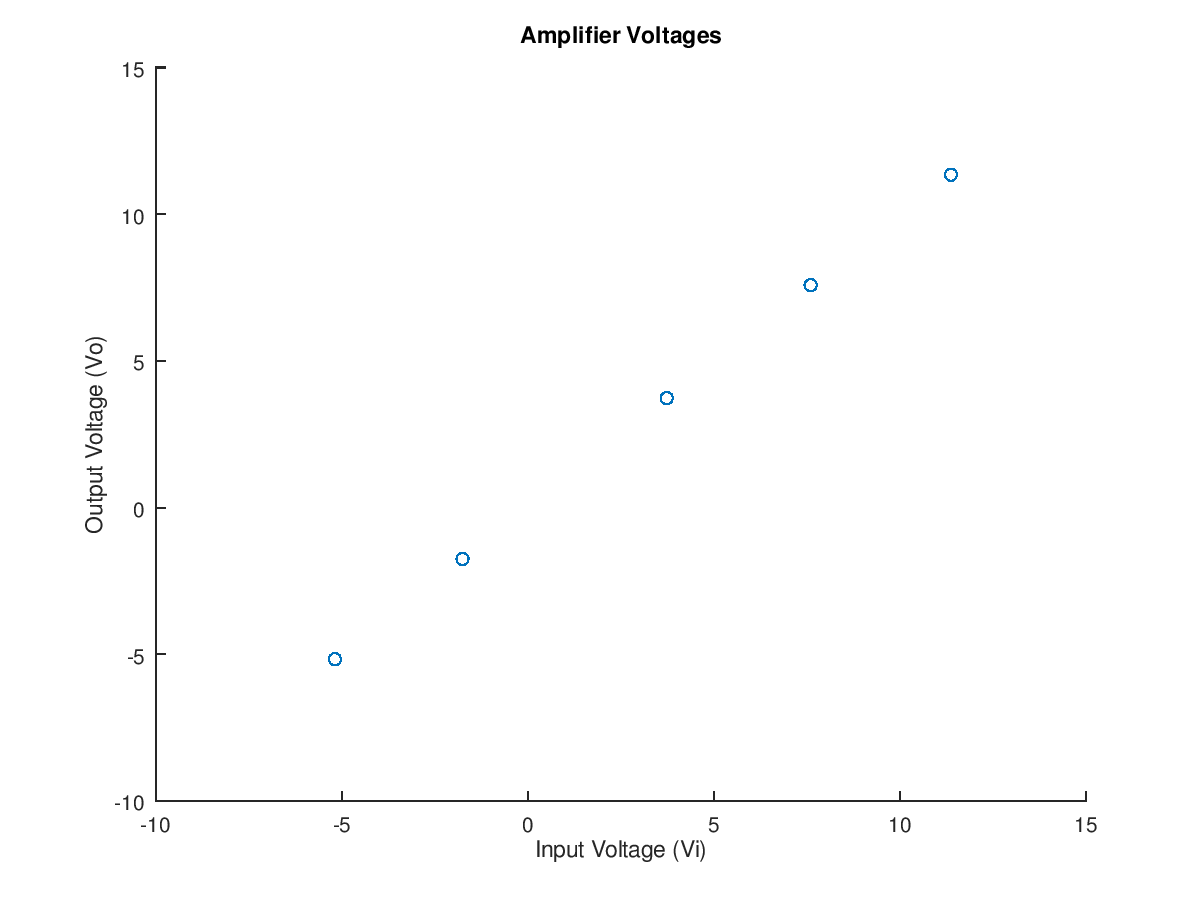
\includegraphics[width=5in]{gainGraph.png}
	\caption{Amplifier Voltage Graph}
	\label{fig4}
\end{figure}

Voltage gain is defined as $\frac{V_{o}}{v_{i}}$. Since this is a graph of $V_{o}$ vs $V_{i}$ we know that the slope of this line should indeed be the gain of the circuit. Throughout the graph the slope appears to remain constant, implying that the gain of the circuit does not depend on the input voltage of the circuit. The same trend can be found in the data collected of the other circuits as well. 

This is a very valuable thing to know, because we would otherwise need to accommodate, in our designs, for a variation based on the input. 

\begin{thebibliography}{99}
% The numeral (here 99) in curly braces is nominally the number of entries in
% the bibliography. It's supposed to affect the amount of space around the
% numerical labels, so only the number of digits should matter--and even that
% seems to make no discernible difference.
Not Requested
\end{thebibliography}

\end{document}
